\subsection{structs und unions}


Als Beispiel sehen wir uns dazu eine Struktur für die ARGB-Farbkodierung an (mit alpha-, rot-, grün- und blauem Farbkanal). 

\cpppInputListing{05_c/problems/listings/channels_struct.c}

%union color beispiel interaktiv gestalten. Folien Willert 02b seite 9-11

Neben structs gibt es auch unions, welche syntaktisch ähnlich sind.
Der Unterschied ist, dass hier die einzelnen Felder vereint werden und sich den gleichen Speicherplatz teilen. 
Verändert man also eine der Variable, ändert sich der gemeinschaftlich genutzte Speicherplatz und der Wert der anderen Variablen entsprechend. 
Demnach ist eine Vereinigung dann sinnvoll, wenn der Wert einer Variablen unabhängig vom Typ gleichviel Speicherplatz benötigt und im selben Speicherbereich abgelegt werden soll.


Die ARGB-Farbcodierung lässt sich statt in 4 einzelnen Variablen auch als eine einzige Integer Variable schreiben, weshalb wir hier eine \lstinline{union} verwenden können.

\begin{figure}[!htb]
	\centering
	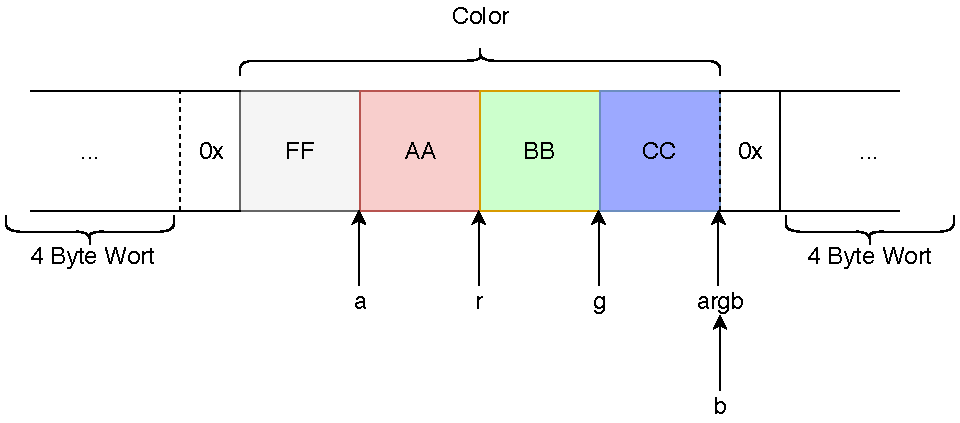
\includegraphics[width=0.6\textwidth]{./05_c/figures/Color_Channels.pdf}
	\caption{Union Color im Speicher}
	\label{fig:color_channels}
\end{figure} 

\cpppInputListing{05_c/problems/listings/union.c}


Lass dir nun die Größe der Variable \lstinline{c}, den Inhalt der Variablen in der \lstinline{union}, sowie die Speicherstellen aller einzelnen Variablen des structs sowie der Integer Variablen mit Hilfe von \lstinline{printf} ausgeben. Was stellst du fest? 

\hints{
\item Mit \lstinline{\%x} kannst du Zahlen in Hexadezimal formatieren.

}